\begin{statementbox}
设椭圆 $E:x^2/a^2+y^2/b^2=1$（$a>b>0$），圆周
$\Gamma:(x-x_0)^2+(y-y_0)^2=r^2$（$r>0$），圆心为 $M$。
本文的“圆”均指\textbf{圆周}，不是圆盘。

\textbf{先看图：外离时，最近距离取差，最远距离取和。}
下图取 $a=2,b=1,M(0,4),r=2$；红段是最近距离，紫色尺寸线标出最远距离。
% E: x^2/4+y^2=1; Gamma: x^2+(y-4)^2=4. Equal metric scale.
\begin{center}
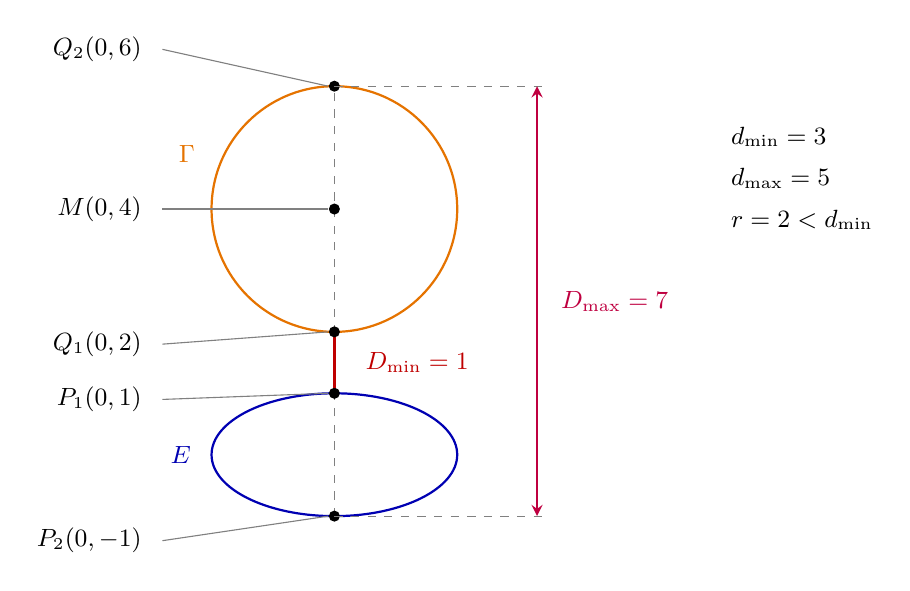
\begin{tikzpicture}[x=.78cm,y=.78cm,>=stealth,font=\small]
\draw[blue!70!black,thick] (0,0) ellipse (2 and 1);
\draw[orange!90!black,thick] (0,4) circle (2);
\node[blue!70!black] at (-2.5,0) {$E$};
\node[orange!90!black] at (-2.4,4.9) {$\Gamma$};
\draw[gray,dashed] (0,-1)--(0,6);
\draw[red!75!black,very thick] (0,1)--(0,2);
\foreach \yy in {1,2,-1,6,4} {\fill (0,\yy) circle(2pt);}
\draw[gray] (-.1,1)--(-2.8,.9) node[left=4pt,text=black] {$P_1(0,1)$};
\draw[gray] (-.1,2)--(-2.8,1.8) node[left=4pt,text=black] {$Q_1(0,2)$};
\draw[gray] (-.1,-1)--(-2.8,-1.4) node[left=4pt,text=black] {$P_2(0,-1)$};
\draw[gray] (-.1,6)--(-2.8,6.6) node[left=4pt,text=black] {$Q_2(0,6)$};
\draw[gray] (-.1,4)--(-2.8,4) node[left=4pt,text=black] {$M(0,4)$};
\node[red!75!black,anchor=west] at (.35,1.5) {$D_{\min}=1$};
\draw[gray,dashed] (0,-1)--(3.5,-1) (0,6)--(3.5,6);
\draw[<->,purple,thick] (3.3,-1)--(3.3,6)
 node[midway,right=5pt] {$D_{\max}=7$};
\node[anchor=west,align=left] at (6.3,4.5)
 {$d_{\min}=3$\\[4pt]$d_{\max}=5$\\[4pt]$r=2<d_{\min}$};
\end{tikzpicture}
\end{center}


记 $d_{\min}=\min_{P\in E}PM$、$d_{\max}=\max_{P\in E}PM$。
两条曲线间的距离最值（$P\in E,Q\in\Gamma$）为
\[
 D_{\min}=\min PQ=
 \begin{cases}
 d_{\min}-r,&r<d_{\min},\\
 0,&d_{\min}\le r\le d_{\max},\\
 r-d_{\max},&r>d_{\max},
 \end{cases}
 \qquad D_{\max}=\max PQ=d_{\max}+r.
\]
\textbf{判断依据：}$PM$ 取遍 $[d_{\min},d_{\max}]$，故
$D_{\min}=\min_{t\in[d_{\min},d_{\max}]}|t-r|$。
$r<d_{\min}$ 时也可能是小圆在椭圆内；不能一概判为外离。
\end{statementbox}
